\documentclass{article}
\usepackage[utf8]{inputenc}
\usepackage{geometry}
\usepackage{natbib}
\usepackage{pxfonts}
\usepackage{graphicx}

\title{Episodic memory: mental time travel or a quantum `memory wave' function?}
\author{Jeremy R. Manning\\Dartmouth College, Hanover, NH\\jeremy.r.manning@dartmouth.edu}

\begin{document}
\maketitle

\begin{abstract}
Where do we ``go'' when we recollect our past?  When remembering a past event, it is intuitive to imagine some part of ourselves mentally ``jumping back in time'' to when the event occurred. I propose an alternative view, inspired by recent evidence from my lab and others, as well as by re-examining existing models of episodic recall, that suggests that this notion of mentally revisiting any specific moment of our past is at best incomplete and at worst misleading.  Instead, I suggest that we retrieve information from our past by mentally casting ourselves back simultaneously to \textit{many} time points from our past, much like a quantum wave function spreading its probability mass over many possible states.  This revised conceptual model makes important behavioral and neural predictions about how we retrieve information about our past, and has implications for how we study episodic memory experimentally.
\end{abstract}

\section*{Introduction and overview}
How do our brains organize, retrieve, and act upon the ceaseless flow of incoming information and experiences?  \cite{Tulv83} contends that episodic memory is like a sort of ``mental time travel,'' whereby we send some part of our mental state back along our autobiographical time line to a specific moment in our past.  This view has fundamental implications for how we study and build theories about memory: it suggests that we can match up specific moments of recollection with specific moments from the past.  These implications extend to how we design episodic memory experiments and how we analyze the behavioral and neural data from those experiments in order to understand the neural and/or cognitive mechanisms that underly memory retrieval.  At its core, characterizing episodic memory as mental time travel makes studying and understanding memory about matching up the thoughts (and/or brain activity patterns) participants are experiencing at one moment with the thoughts (and/or brain activity patterns) participants experienced at another previous moment.  The challenge, then, is to understand the neural (structural) and cognitive (functional) mechanisms that characterize when, how, and why our memory systems allow us to relive those prior experiences.  One way of illustrating how this framing misses out on key aspects of memory is to examine how experimentalists and theorists typically conceive of and model a mental construct called \textit{context}.

The notion of context was fundamental to \citeauthor{Tulv83}'s characterization of episodic recall, and continues to be a primary feature of most current theories of episodic memory~\citep[e.g., for review see][]{Kaha12}.  Whereas the \textit{content} of a memory provides specific information about the episode itself, contextual components of a memory help to frame the episode within the rememberer's broader experience.  Defining context precisely (e.g., as distinct from content) is an ongoing challenge for our field, but theorists generally describe context as reflecting a mental combination of external cues (where you are, who you are with, background sensory information, etc.) and internal cues (thoughts, feelings, emotions, etc.) that uniquely define each moment~\citep[e.g., see review by][]{MannEtal15}.  Reactivating the mental representation of the context associated with a given episode is what can give us the feeling of some ``part of ourselves'' re-experiencing the past.

One practical way to distinguish content from context representations is to separate mental (or neural) representations that drift rapidly \citep[content;][]{PolyEtal05, MannEtal12} or gradually \citep[context;][]{PolyEtal05, MannEtal11, HowaEtal12, LohnEtal18, LongKaha18, FolkEtal18}.  An intuition for why contextual representation might be expected to evolve gradually is laid out by \cite{PolyKaha08}.  Essentially, slowly drifting thoughts may be used to ``index'' more rapidly drifting thoughts that are temporally proximal.  This notion, that our brain maintains parallel mental representations drifting at different time scales, has been well-characterized in a series of elegant fMRI and ECoG studies by Uri Hasson and colleagues~\citep{HassEtal08, LernEtal11, HoneEtal12, AlyEtal18}.  Subsequent work by the same group has shown that this hierarchy of drifting mental representations plays a central role in how we remember continuous experiences and segment our experiences into discrete events~\citep{BaldEtal17}. This work mirrors the discovery of \textit{time cells} in the rodent hippocampus that respond preferentially to a specific time relative to a temporal reference, whereby each cell appears to integrate incoming information at a different rate~\citep{PastEtal08, MacDEtal11}. Recent work also suggests that the lateral entorhinal cortex plays a role in integrating information across a wide range of timescales~\citep{TsaoEtal18}.  These ideas have been formalized in a family of theoretical models over the past several decades~\citep{HowaKaha02, DianEtal07, SedeEtal08, PolyEtal09, ShanEtal09, ShanHowa10, ShanHowa12, HowaEtal14}.  In turn, these models were inspired in part by earlier theoretical work suggesting that temporally proximal experiences become linked through their shared contextual features~\citep{Este55a,AtkiShif68}.  Collectively, these experimental and theoretical studies make two important contributions to our understanding of how we remember our past.  First, the studies suggest that our ongoing experiences are ``blurred out'' in time by neural integrators (where different brain structures or sub-structures integrate with different time constants).  Second, the studies suggest that members of this family of representations drifting at different rates become bound together such that when we retrieve memories about our past, we reactivate representations that carry information at a range of time scales.  These reactivations explain how our brains reactivate prior contexts when we remember the past.

Although reactivating context is often \textit{described} as a sort of mental time travel back to the one specific moment being remembered, there is some apparent inconsistency between this description and how this process is actually characterized mathematically or measured neurally.  In particular, both the theory and neural measures described in the preceding paragraphs characterize episodic recall mathematically as reflecting the reactivation of a weighted blend of thoughts from a \textit{range} of previously experienced times-- not to any one \textit{specific} time.  This is not simply a matter of imprecision in mental time travel (i.e., a reflection of the low effective resolution with which we can revisit specific moments from our past).  Rather, when we retrieve the thoughts associated with a range of times, it is conceptually more like we are simultaneously visiting \textit{many} of our prior experiences. The above human and rodent studies suggest that the brain maintains parallel representations of ongoing experience, each drifting at a different timescale.  The notion of thinking of any one particular moment from the past is incompatible with this multiple timescales view, in that our thoughts and brain activity patterns reflect information from a range of moments, even when we are not specifically engaged in remembering.  If what we consider to be a ``moment'' or ``now'' is guided by our neural representations of our ongoing experiences, then this implies we are continually experiencing \textit{many} ``nows.''  If our thoughts are continually spread across a range of times, the notion of mentally revisiting any particular moment loses its meaning.

Where the mental time travel framing breaks down most notably is when we consider scenarios in which the particular blend of timepoints reflected in one's current thoughts do not come from temporally contiguous events.  For example, understanding how a new experience fits in with our broader understanding might require integrating information gleaned from many experiences separated in time, each with their own contextual attributes.  That we can integrate information across experiences suggests that the integration of incoming information at different rates need not be a purely mechanical process, but rather may reflect a deeper functional role.  When we simultaneously reactivate thoughts related to separated moments from our past, this provides a means of associating and relating those temporally distinct experiences.  This is how we can integrate information across the \textit{many} discrete experiences relevant to ``now.''

\section*{The temporal dynamics of ongoing experience and how we remember it}
Modern context-based theories of episodic memory posit that the current state of mental context serves to determine which information from our past may be relevant to us and therefore reactivated~\citep[e.g., ][]{PolyEtal09}. Although these theories were largely developed and tested in the domain of list-learning paradigms, conceptually similar principles might also underlie real-world memory.  For example, prior experiences with shared or overlapping contextual properties (e.g., other experiences that occurred in similar spatial or social settings, shared similar goals, etc.) could be leveraged to form schemas or situation models that help guide behaviors and expectations according to the current perceived context~\citep{RangRitc12, BaldEtal18, AlyEtal18}.

Unlike random word lists, naturalistic experiences contain \textit{event boundaries} whereby contextual cues change sharply from one moment to the next, implying a change in the current situation (e.g., shifting from the quiet peace of working on a manuscript in the early morning to the different peace of helping a newly awoken child get ready for school).  A number of studies (using non-random lists and more naturalistic stimuli) have found that the way we remember past experiences can be shaped by these event boundaries.  For example, controlling for elapsed time, memory is impaired for information that occurred prior to a change in the current event or situation~\citep[e.g., ][]{RadvCope06, SwalEtal09, SwalEtal11, EzzyDava11, MannEtal16}.  The temporal dynamics of contextual change also underlie how we judge the amount of time elapsed since a prior reference point~\citep{BlocReed78, SahaSmit14}.  These findings suggest that the rapid contextual or situational changes that define these event boundaries shape how we experience and remember, similarly to how spatial boundaries~\citep[e.g., environmental barriers;][]{McKeBuzs16, BrunEtal18} shape how we experience and remember spatial environments and layouts, or how conceptual boundaries~\citep[e.g., distinctions between semantic categories;][]{BrunEtal18} shape how we experience and remember conceptual information.

Event boundaries are one example of the broader temporal covariance structure that is characteristic of ongoing experience.  Whereas classic approaches to studying memory (e.g., list-learning paradigms and other trial-based experiments) encourage researchers to treat each moment, trial, or stimulus as separable from the rest of experience, context-based theories of memory (including situation models and event-based models) posit that each moment derives meaning through its deep ties to other experiences.  This rich tapestry of interacting moments and experiences forms the scaffolding for interpreting our new experiences and for retrieving information concerning our past.  According to this view, the reactivation of this rich tapestry of contextual details enfolding the remembered event (i.e., how the event relates to the rest of ones experiences across timescales) is even more central to our subjective experience than the specific details of what occurred during that event!  This begs the question: which thoughts, from which times, do we reactivate when we remember our past experiences?

\subsection*{How is our past replayed when we remember?}
Our ongoing experiences can cue us to dredge up information about our past.  This can happen explicitly (e.g., during a conversation about a prior event) or implicitly (e.g., when something happening now reminds you of what happened before).  Context-based theories of memory posit that the particular memories that our ongoing experiences cue will be related~\citep[contextually, semantically, functionally, etc.; e.g., ][]{PolyEtal09}.  One potential challenge to studying how we remember the past relates to detangling which links between our experiences are specifically driven by our memory systems versus which are imposed ``externally'' through the similarity structure of those experiences.  For example, consider your daily commute into work.  If you were to verbally recount a specific day's commute later, one might expect some aspects of your description to apply to other days' commutes as well (e.g., other commutes where you took a similar route or travelled via similar modes of transportation, listened to similar music along the way, travelled at a similar time, etc.).  But to what extent could one hope to separate out descriptive matches driven solely by similarities in those commuting experiences, versus true reactivations (in memory) of specific memories of those other prior commutes?

Once insight into this distinction comes from a recent study by \cite{HeusEtal18c}, which analyzed data collected by \citep{ChenEtal17} who had participants watch an episode of the BBC television show \textit{Sherlock} and then verbally recount what happened in the episode.  The authors used topic models~\citep{BleiEtal03} applied to human annotations of each camera shot in the episode to characterize the episode's content with a timeseries of high-dimensional semantic feature vectors.  When characterized in this way, the episode's content exhibits periods of relative stability, followed by moments of rapid change. This interplay between stability and change is visible as ``blocks'' in the temporal correlation matrix (Fig.~\ref{fig:corrmats}A); \citep{HeusEtal18c} perform detailed analyses of these putative events and how they are remembered.  Notably, the off-diagonal entries of the temporal correlation matrix (which reflects content similarity between temporally distant events in the episode) are nearly all close to 0.  This is surprising, because the episode itself comprises a murder mystery with recurring motifes that must be associated in the viewer's mind in order to make sense of the episode.  Nonetheless, when considering solely the semantic content of each moment of the episode, those long timescale associations are nearly entirely absent.  To the extent that this finding extends to real-world experiences, it comports with Heraclitus' notion that one cannot step in the same river twice~\citep{Hera}.

\begin{figure}[tp] \centering 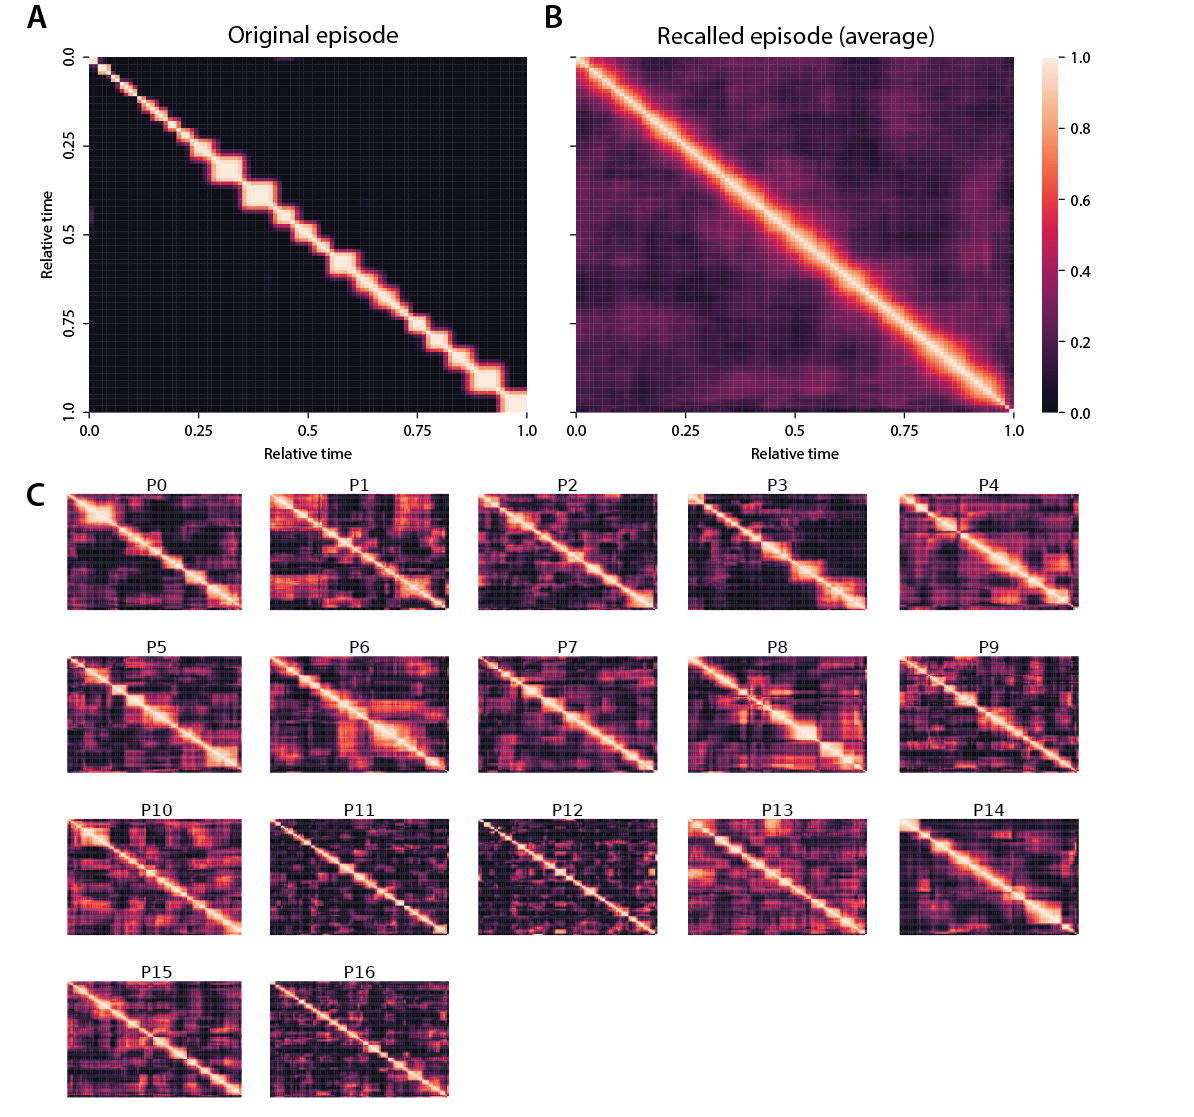
\includegraphics[width=\textwidth]{figs/pres_rec_corrmats_sherlock} \caption{\textbf{Temporal correlation matrices of the dynamic content of a television episode and people's recalls of that episode.}  The panels of this figure are adapted from \cite{HeusEtal18c}, where full details may be found. \textbf{A. Temporal correlations exhibited by the content of the television episode.}  Each moment of an episode of the BBC television show \textit{Sherlock} has been characterized using a topic model~\citep{BleiEtal03} fit to detailed human-generated annotations of each scene cut.  The correlations between the topic vectors of a given pair of timepoints reflects the similarity in content between those timepoints.  \textbf{B. Temporal correlations exhibited by the (average) content of participants' recalls of the episode.} The topic model used to characterize the episode in Panel A has been applied to each sentence, from each participants' recall transcript.  The temporal correlation matrices describing each participants' recalls were re-sampled using cubic interpolation to have 100 rows and columns prior to averaging the resampled matrices across participants.  \textbf{C. Temporal correlations in the content of individual participants' recalls of the episode.} Each sub-panel displays the temporal correlation matrix for one experimental particpant.}
\label{fig:corrmats}
\end{figure}

Although the specific content of each moment of the episode is largely unique, participants' subjective experiences of the episode entail weaving together those temporally separated moments into a cohesive narrative.  This is reflected in how people verbally recount the episode later.  If we examine the temporal autocorrelation matrices of participants' recalls of the television episode (characterized using the same topic model used to capture the content of the episode; Figs.~\ref{fig:corrmats}B, C), we see a different structure than that of the episode itself.  Although individual participants' recalls exhibit periods of content stability punctuated by rapid change (block diagonal structure of the matrices in Fig.~\ref{fig:corrmats}C), the off diagonal correlations between temporally distant events are substantially stronger in participants' recalls than in the original episode.  Another way of characterizing this phenomenon is to look at the autocorrelation functions (describing the correlation between different moments' topic vectors as a function of their temporal distance) for the episode and participants' recalls (Fig.~\ref{fig:reinstatement}A).  Whereas the autocorrelations for the original episode rapidly fall to 0, autocorrelations in the content of participants' recalls appear to asymptote around 0.2.  These analyses indicate that the way participants \textit{recount} temporally separated events imposes additional similarity on those events, beyond what was present in the original events themselves.  One can then ask: is this simply a matter of imprecision in recall, either with respect to participants' recalls themselves, or with respect to the quality with which they are characterized via semantic feature vectors?  Or might there be a functional role to that additional imposed similarity structure?

To examine which specific events are described (during recall) as more similar than what their original experiences (as characterized by semantic feature vectors) would suggest, it can be helpful to examine individual recalls of particular events throughout the episode.  Figure~\ref{fig:reinstatement}B displays, for a representative example recalled moment, which other moments from the episode were described in a similar way by the participants when they recounted the episode later (black and colored lines), and which other moments in the episode were described in a similar way in moment-by-moment (non-recall) human annotations (gray line).  The example event explored in the figure comprises a scene where Sherlock Holmes and John Watson (main characters) are bantering, and then are interrupted when Sherlock realizes that another victim has been murdered.  The language used by human annotators describing the moment-by-moment contents of the scene used a similar mix of themes only for moments in the episode that were temporally proximal to the event in question (gray line).  However, the way participants \textit{described} what happened when they recounted the episode later revealed a much different pattern.  Specifically, their language mirrored that used when they were recalling other murders, and other moments when Sherlock and John were bantering (Fig.~\ref{fig:reinstatement}C).  Further, the way they described this example event did \textit{not} mirror the way they described other semantically (but not conceptually) related events, such as events involving unrelated violence, or Sherlock and John interacting with other characters.  Taken together, this suggests that these specific events were associated in participants' memories, perhaps contributing to (or reflecting) their understanding that those events were linked in the episode's narrative.

\begin{figure}[tp] \centering 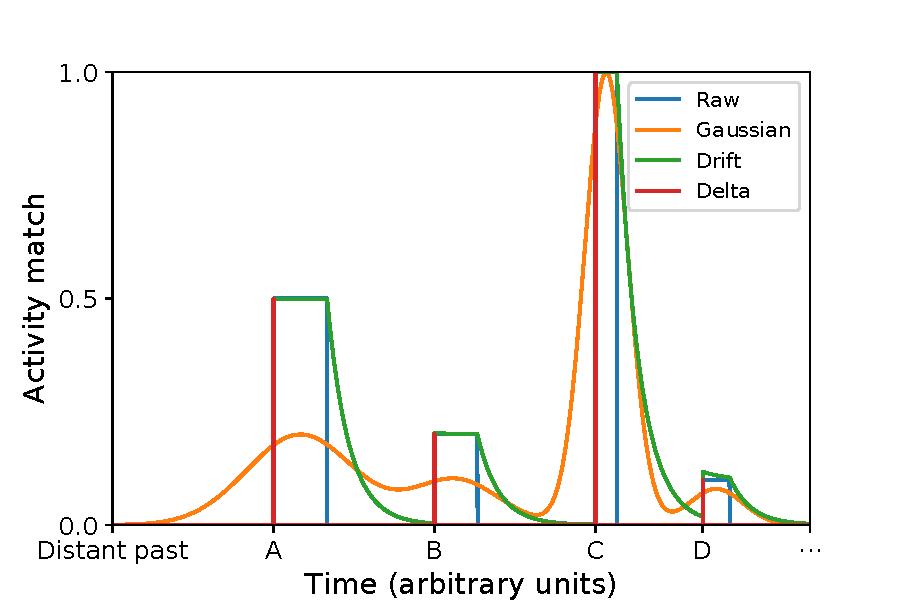
\includegraphics[width=\textwidth]{figs/reinstatement} \caption{\textbf{Content drift in a television episode and participants' recalls of that episode.  A.  Autocorrelations in the episode's content and in the content of participants' recalls.}  The black line denotes the average correlations between the topic vectors from pairs of moments in the episode as a function of their temporal separation (times are relative to the full length of the episode).  Each colored line denotes an analogous autocorrelation function, but for each individual participant's recalls of the episode (times are relative to the full length of each participant's recalls).  The error ribbons denote 95\% confidence intervals, taken across all moments in the episode (or in participants' recalls of the episode).  \textbf{B. Recall density functions for one recalled moment.} Each curve reflects the correlations between the topic vector at each (relative) moment of the episode (or participants' recalls of the episode), and the topic vector of an event beginning approximately $\frac{1}{3}$ through the episode (relative time: 0.328).  The gray curve denotes these correlations for the topic vectors derived from annotations of the episode itself. The black line denotes the average correlations across all participants' recalls.  Local maxima are marked with colored dots.  Local maxima closer than 2.5\% of the total recall duration to a higher local maximum were excluded, as were maxima with peaks with correlation coefficients lower than 0.1 (arbitrarily chosen; these ).   The colored lines denote the correlations for each individual participant's recalls.  \textbf{C. Local maxima in the average recall density function.}  Representative screen captures from the scenes at each local maxima in Panel B are displayed (dot colors match those in Panel B).  The text in each screen capture displays a brief summary of what happened in each scene.}
  % colors: individual participants
  % black: average across participants
  % gray: autocorrelation with topic vector at timepoint
  % circles: local maxima in the across-participants average (i.e., movie events that share structure with the given timepoint that is distinct from other temporally proximal events)
\label{fig:reinstatement}
\end{figure}

A rich recall density function analogous to the one displayed in Figure~\ref{fig:reinstatement}B could, in principle, be characteristic of memory for \textit{any} past event or experience.  For example, the peaks of the function could provide insight into which events, from which moments along one's autobiographical timeline, were functionally associated in memory.  Nonetheless, a potential challenge to testing this hypothesis in the laboratory is that in most memory studies there is no particular reason for participants to functionally associate the stimuli-- there is no ``deeper narrative'' to make sense of.  However, random word list learning experiments might happen to contain (for a given list) semantically related words.  And indeed, a number of studies indicate that participants spontaneously form associations between semantically related words on random word lists, even when those related words are separated in time~\citep[e.g.,][]{WixtRohr94, MannKaha12, MannEtal12}.  This suggests that our memory systems pick up on statistical regularities, even in ostensibly ``random'' stimulus sequences, and that we leverage those regularities when we recall our past~\citep{PolyEtal09}.  Other work suggests that our memory systems may also leverage these regularities to parse our ongoing experiences into discrete events~\citep{SchaEtal13}.  Are these examples in the literature on random list learning studies, indicating that our memory systems leverage ``accidental'' structure in random sequences, a reflection of the same fundamental principle driving the sorts of memory reactivation function displayed in Figure~\ref{fig:reinstatement}B?

It is difficult to explicitly test whether (apparent) semantic reinstatement in word list learning, as reflected in people's tendencies to semantically cluster recalls of random word lists, reflects integration of information across the experiences of studying those words.  However, remembering word lists does not \textit{require} integrating information across words in order to specifically gain a deep understanding of the list.  By design, there \textit{is} no deeper meaning of random word lists.

\textbf{JRM STOPPED HERE}

\section*{BRAINSTORMING OUTLINE OF THE REST OF THE PAPER}
\begin{enumerate}
  \item \textit{Show video correlation matrix + recall correlation matrix.  Key idea: off-diagonal mass is introduced (primarily) by how people \textit{remember} the movie, not due to the contents of the movie itself (evidence: correlation matrices).  Further, this is not simply a matter of imprecision in how people recall, and/or our approach's ability to characterize recalled events (evidence: reinstatement figure showing which scenes are recalled similarly).  This sort of integration is how we ascribe meaning to events that unfold over disjointed extended timescales.}
  \item \textit{In theory this could also happen during \textit{any} sort of experience.  For example, when people study random word lists, they often re-order their recalls so that semantically related words are closer in the recall sequence than they were in the presented sequence.  This can be captured to an extent by semantic clustering measures.  However, it's difficult to examine this phenomenon in more depth because word lists necessarily lack the richness of more naturalistic stimuli.  There are no ``deeper ties'' between study events (i.e., individual words), so the sorts of integration operations that allow us to make sense of real-world experiences aren't given the same freedom of expression in list-learning experiments.  Evidence: presentation/recall correlation matrices during random free recall don't show the same sort of off-diagonal increase.}  Claim: mental time travel and quantum wave reinstatement look the same for random word list remembering, but very different for real-world remembering.
  \item The specific ties between unfolding events forms a scaffolding for understanding how those events are related.  This can be visualized geometrically by projecting word embedding representations of the events onto lower dimensional spaces (although see Flatland Fallacy paper, with HyperTools paper as a potential counterpoint).  This reveals another key property of how we remember: although there are substantial individual differences in the specific words people use to describe a shared experience, and how much detail they get into, the overall ``shapes'' of those recalled experience trajectories are highly similar across people.  This has potentially exciting implications for how we communicate memories to other people: we need to convey the ``gist'' (shape) of our experience.  It also has implications for how we learn by analogy: perhaps events that share schemas (cite Baldassano et al) unfold in similar ways (e.g. have similar shapes).  Learning which shapes go with which schemas could provide a scaffolding for rapid learning and generalization of new experiences, to the extent that those new experiences match a previously learned schema (shape).
    \item These ideas also have implications for other forms of learning (e.g. spatial learning) and neural decoding.  When we attempt to characterize thoughts (e.g. training a classifier to distinguish between states), we tend to train decoders to estimate the ``one'' state that the brain is in.  However, perhaps we should instead consider that our brains are contemplating, or holding in our thoughts, many possible states simultaneously.  Therefore we should consider the full distribution of states (rather than only considering its maximum) as a primary metric of characterizing mental function.  (Probably people have proposed this-- e.g. representing the posterior and using it to compute...need citations.)
    \end{enumerate}

\textbf{KEY QUESTIONS}:
\begin{enumerate}
  \item Is this more of a ``review'' paper, or should I highlight the new analyses more?
  \item Who is this paper alienating and how can the narrative be reframed in a more inclusive way?
  \item Which ideas are ``new'' vs. restatements of old ideas?
  \item What are the key testable predictions to highlight, and how can they be communicated most clearly and effectively
  \item What's an appropriate venue for this?
\end{enumerate}

\section*{How do our experiences and memories unfold over time?}
Although real-world experiences can exhibit rich temporal structures, it can be illustrative to consider the transformation of how we experience much simpler and less naturalistic events (e.g. studying random word lists) versus how we later remember those experiences.  Figure~\ref{fig:corrmats}A displays an average temporal correlation matrix describing the similarity structure of 1072 random word lists, each comprising 16 words~\citep{ZimaEtal18}.  I applied a topic model (trained on a curated corpus of Wikipedia articles) to yield a 100-dimensional embedding of each presented word~\citep{BleiEtal03}.  The left panel displays the average correlations between the topic vectors of each pair of presented words as a function of their presentation positions.  As shown, nearly all of the correlation ``mass'' is along the diagonal, and the off-diagonal entries are very close to zero.  Because the word orders were randomized, the temporal correlation matrix reflects that there are no consistent similarity patterns between any given pair of timepoints.  The right panel of Figure~\ref{fig:corrmats}A displays the average temporal correlation matrices describing participants' \textit{recalls} of those same lists.  Although the recall matrix exhibits the strongest correlations along its diagonal, some correlation mass bleeds into nearby recalls, reflecting (in part) participants' tendancies to recall semantically related words successively.\footnote{Note that participants recalled different numbers of words from each studied list; I used linear interpolation to resample each recall correlation matrix that preserved the size of the presentation correlation matrix.  This process resulted in some additional blurring along the diagonal.  In other words, the blurring along the diagonal reflects two phenomena: participants' tendancies to semanticly cluster their recalls, and an artifact of the temporal resampling.}  Differences in the temporal correlation structure between the original lists of words and the orders of participants' recalls illustrate one way that our memory systems can reorganize our experiences such that we recall them in a different way than we originally experienced them.








\textbf{JRM NOTE: add section on the temporal structure of list-learning vs. naturalistic stimulus, and on the temporal structure of recalls.}

\section*{The shapes of remembered experiences}
In a recent study~\citep{HeusEtal18c} my lab examined functional neuroimaging and behavioral data collected by \cite{ChenEtal17} as participants viewed and then verbally recalled an episode of a television show.  We used topic models~\citep{BleiEtal03} to characterize the moment-by-moment content of the episode and of participants' recalls.  Each moment was quantified via a \textit{topic vector} that reflected the mix of topics (themes) the model identified in that moment.  In this way, the sequence of topic vectors over the course of the episode traces out a \textit{topic trajectory} through a high-dimensional feature space.  The sequence of topic vectors for a given participant's recalls traces out an analogous trajectory.  This characterization provides a geometric framework for comparing the \textit{shapes} that reflect how naturalistic experiences unfold over time, to the shapes of how we remember those experiences later (Fig.~\ref{fig:trajectories}).  One can then use the geometric transformations needed to map an experience's trajectory onto the trajectory of its later remembering to characterize the quality and content of memory.

\textbf{JRM STOPPED HERE}

\begin{figure}[tp]
\centering
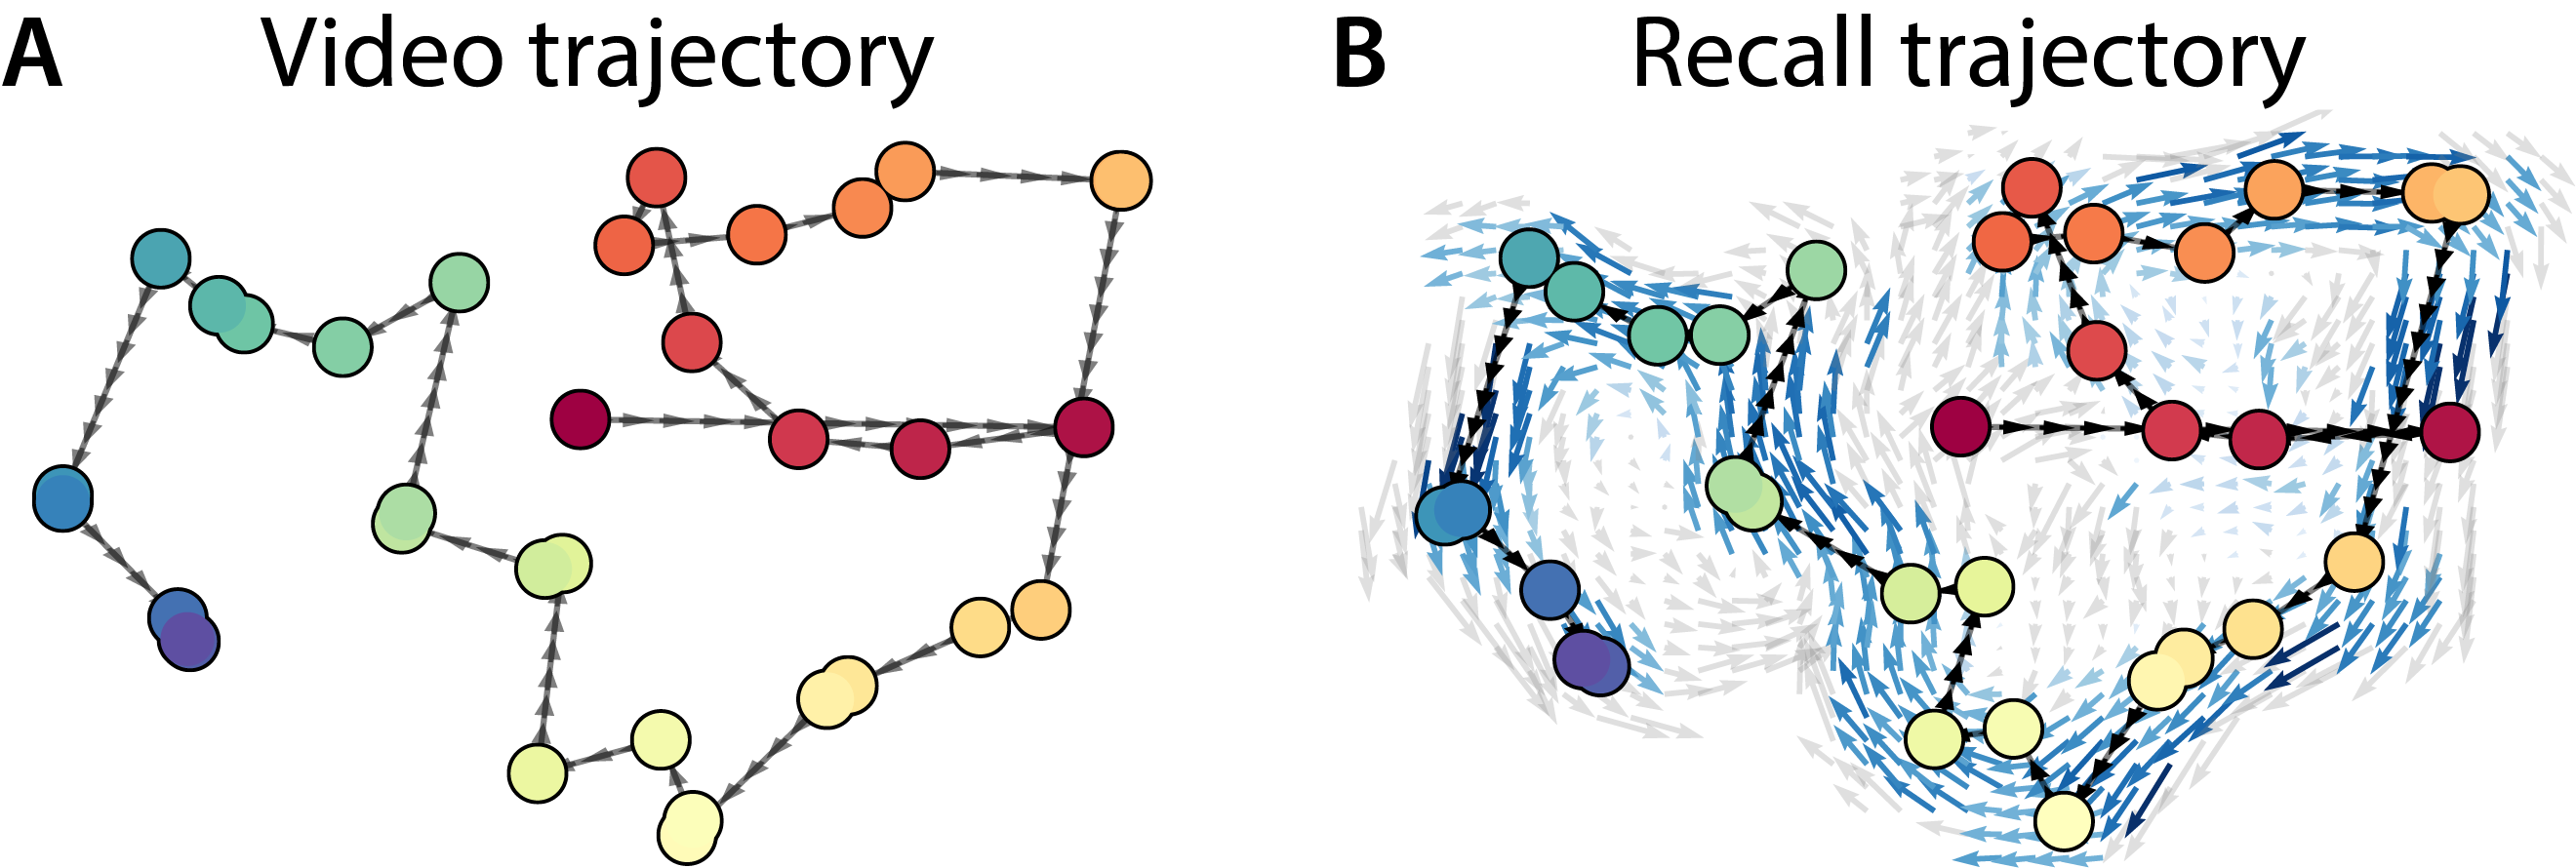
\includegraphics[width=0.8\textwidth]{figs/trajectory}
\caption{\textbf{Topic trajectories of a video and its memory.}  \textbf{A.} The topic trajectory taken by a 50 minute television episode, projected onto two dimensions.  Each dot indicates an event identified using a Hidden Markov Model; the dot colors denote the order of the events (early events are in red; later events are in blue), and the connecting lines indicate the transitions between successive events.  \textbf{B.} The average two-dimensional trajectory captured by 17 participants' recalls of the episode, with the same format and coloring as the trajectory in Panel A. The arrows reflect the directions of the average transitions taken by participants whose trajectories crossed that part of topic space; blue denotes reliable agreement across participants.  Figure adapted from \cite{HeusEtal18c}.}
\label{fig:trajectories}
\end{figure}



defines a distinction between the gist


\begin{itemize}
\item Not about the number of details-- it's about capturing the overall ``shape'' of past experience
\item Quantifying recall should be about the match between the shape of the original experience (i.e., the covariance structure describing how it unfolds over time), not about the number of details that are recovered
\item When we retrieve memories, we cast ourselves along the full trajectory simultaneously (perhaps covering each component to a different degree), not to a single point (moment)
\item Predictions:
\begin{itemize}
    \item What makes an effective summary?  One that efficiently captures the overall shape of the experience.
    \item How do we communicate our experiences to others?  Describe the path through conceptual space.
    \item How do we communicate our experiences to our ``future selves?''  Describe the path through conceptual space.
    \item Each of these notions is fundamentally about the full trajectory, not about a single point.  Each moment derives meaning only in the context of the rest of experience.
\end{itemize}
\item What can list learning tell us?  We get fine control over  contextual representations at a very limited set of timescales.  We can study the detailed impacts of manipulations on memory.
\item What can't list learning tell us?  We can ask whether people precisely reproduce their prior experiences.  But we can't know whether they recover the ``gist'' of those experiences, since random lists do not have meaningful gists.
\item Other thoughts (from previous brainstorms):
    \begin{itemize}
    \item Reactivated neural representations that seem like noise should actually have predictive power for later memories if they get incorporated into the mental state at the time of remembering.
    \item List learning experiments and other experiments with discrete trials are not well equipped to study time spreading because they effectively impose event boundaries around and between every stimulus presentation.  Rather, we need continuous naturalistic recall experiments to more accurately reflect how our brains operate in the real world.
    \item say something about slow drift vs. reinstatement (cite MannEtal11 and FolkEtal18)
    \item something about schema learning (related to semantic memory?) and how memories are compressed (Chen et al 2017, Baldassano et al 2017, 2018) and transmitted to others
    \end{itemize}
\end{itemize}


Our brains exhibit autocorrelated activity.  In the extreme this is trivially true; our brains are biophysical systems that cannot change infinitely quickly, so neural activity patterns are necessarily similar (to some extent) from one moment to the next.  However, autocorrelated activity patterns \textit{at the time scales we typically examine in laboratory memory studies} are far stronger and persist for far longer than is strictly necessary from a biophysical standpoint.  For example, transient changes in neuronal membrane potentials during action potentials can last just a few milliseconds~\citep{HodgHuxl52} and even local field potentials that reflect the synchronized activities of tens of thousands of neurons can exhibit millisecond timescale changes~\citep{Frie05, Buzs06}.  Nevertheless, our brain activity pattern can remain reliably autocorrelated at timescales of seconds or longer-- and these long timescale autocorrelations predict how our ongoing experiences are remembered later~\citep[e.g.][]{MannEtal07, MannEtal11, HowaEtal12, FolkEtal18}.

\section*{Implications}
\subsection*{Extensions to spatial and semantic memory}
Just as we mentally spread ourselves across a distribution of times, we can perform similar mental operations when we conceptualize and retrieve other types of information.  For example, consider how we use pattern classifiers to connect neural activity patterns to specific semantic~\citep{PolyEtal05, MitcEtal08, MannEtal12} or spatial~\citep{MillEtal13} content being mentally manipulated.  The prevailing approach is to label specific brain activity patterns as each reflecting \textit{one particular} semantic concept or spatial location.  Variability in neural activity over repeated experiences or rememberings can result in classifiers spreading their predictions over multiple possible mental states.  Traditional approaches then ``clean up'' this distribution over possible mental states by taking its expected or maximum value.  However, following the ``quantum wave function'' logic, I suggest that the specific shape of these distributions may not only be informative, but they are \textit{more accurate reflections of what our neural activity patterns actually reflect}.

\section*{Concluding remarks}

\bibliographystyle{apa}
\bibliography{CDL-bibliography/memlab}
\end{document}
